\section{Background}

This paper takes the API and load balancers designed in
Mantle~\cite{sevilla:sc15-mantle}, the programmabile file system metadata load
balancer for Ceph, and applies them to
HXHIM~\cite{greenberg:hotstorage2015-mdhim}, the distributed key-value store
designed for HPC.

\subsection{Mantle: File System Metadata Load Balancer}
\label{sec:mantle}

% What is Mantle?
Mantle is an API that lets admnistrators control file system metadata load
balancing. Mantle speeds up file systems by making metadata access faster,
leveraging the fact that file system metadata IO imposes small and frequent
accesses on the underlying storage system. Since data IO does not scale like
metadata IO~\cite{roselli:atec2000-FS-workloads}, finding optimal ways to
measure, migrate, and partition metadata load is a relatively new field, but
has been shown to lead to large performance increases and more scalable file
systems~\cite{zheng:pdsw2014-batchfs, grider:pdsw2015-marfs,
ren:sc2014-indexfs, patil:fast2011-giga+, brandt:msst2003-lh}.  Mantle can use
strategies from these papers to control how to distribute or concentrate file
system metadata.

% How does it work?
It was built on CephFS, the file system above Ceph, so it inherits many of
characteristics of the CephFS architecture, like the dedicated metadata cluster
and heartbeat mechanisms shown at the top of Figure~\ref{fig:arch-mantle}.
Each metadata server manages differently sized subtrees of the logical
namespace and migration decisions are made synchronously, every 10 seconds.
CephFS already had the mechanisms for load balancing, namely the ability to
measure the load on a subtree, to migrate subtrees, and to partition subtrees
into smaller subtrees, but it had hard-coded, ad-hoc policies for guiding the
migrations.  Mantle reads user-defined policies written in Lua and returns
decisions for how load should be migrated given the state of the cluster and
the behavior of the workload. The hooks in Figure~\ref{fig:arch-mantle} show
where CephFS calls out to the Mantle library to make decisions. While the
decisions were made by Mantle, CephFS used its internal mechanisms to do the
load balancing.

% The actual policies
The Mantle paper implemented three balancers and tested them under
metadata-intensive workloads. The Greedy Spill balancer, which was based
on~\cite{patil:fast2011-giga+}, sheds have its load aggressively when there are
avaiable servers. Part of the Lua code for implementing this balancer is shown
in~\ref{fig:arch-mantle-example}.  The Fill and Spill balancer, which was based
on~\cite{pai:asplos1998-lard} sheds a fraction of the load only when the server
is overloaded. Finally, the Adaptable balancer, which was based
on~\cite{weil:sc2004-dyn-metadata, weil:osdi2006-ceph}, sheds a fraction of the
load frequently.

% What is the status?
It was merged\footnote{https://github.com/ceph/ceph/pull/5155} and is starting
to get users who are frustrated with the hard-coded load balancing policies
that are shipped with CephFS. It was re-implemented using the ``programmable
storage" approach~\cite{sevilla:eurosys17} to reduce lines of code for doing
things like versioning and distributing balancer version.  Although Mantle is
heavily integrated the daemons that compose an Ceph cluster, using Ceph's
naming conventions and internal libraries like Ceph's version of protocol
buffers, there is no reason that it cannot be extracted.

\begin{figure}[tb]
  \noindent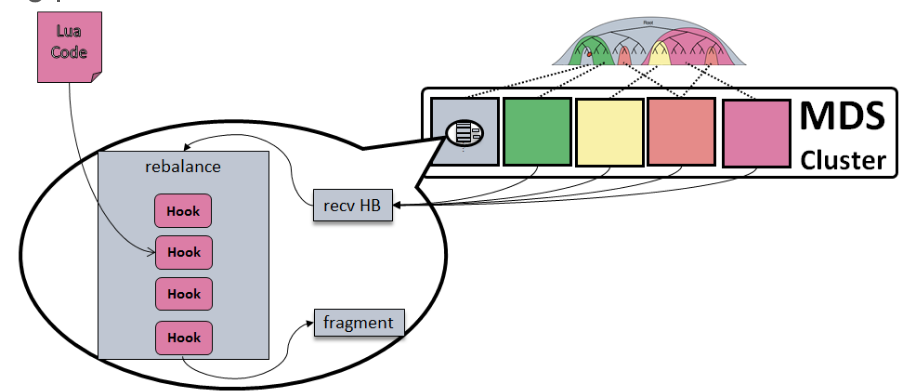
\includegraphics[width=19pc,angle=0]{figures/arch-mantle.png}\\
  \caption{The Mantle API lets adminstrators control load balancing by
  changing the poicies for how to distribution or concentrate file system
  metadata. It was merged into CephFS and inherits many aspects of that
  architecture. Although it has the load balancing structure and logic from
  CephFS (gray boxes), the actual API is not dependent on that code base.}
  \label{fig:arch-mantle}
\end{figure}
\begin{figure}[tb]
  \noindent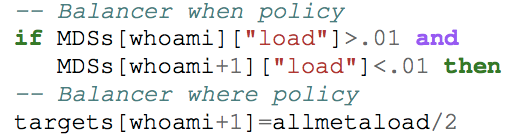
\includegraphics[width=19pc,angle=0]{figures/arch-mantle-example.png}\\
  \caption{The Greedy Spill balancer written in Lua using the Mantle API.}
  \label{fig:arch-mantle-example}
\end{figure}

\subsection{HXHIM: Key-Value Store for HPC}
\label{sec:hxhim}

\begin{figure}[tb]
  \noindent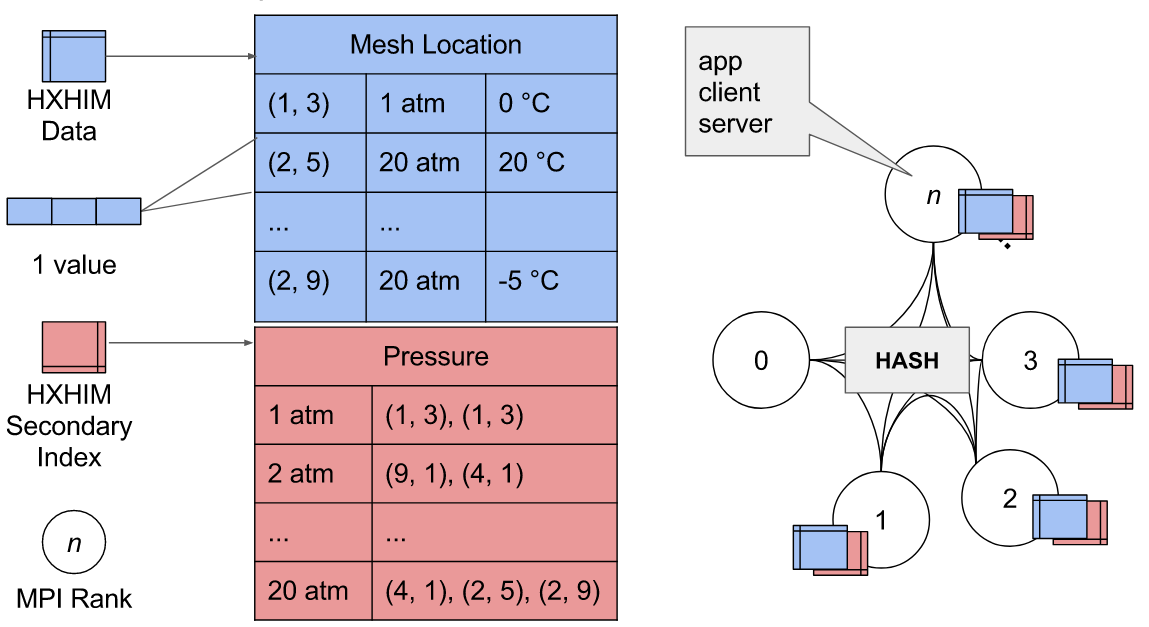
\includegraphics[width=19pc,angle=0]{figures/arch-hxhim.png}\\
  \caption{The HXHIM architecture.}
  \label{fig:arch-hxhim}
\end{figure}

% What is HXHIM
HXHIM is a key-value store designed for HPC architectures and multi-dimensional
data. 

% Why do they make sense together?
% HXHIM has operations for:
% - adjusting the distribution of keys
% - builk inserations/retrievelas

\subsection{Comparing Mantle and HXHIM}
\begin{figure}[tb]
  \noindent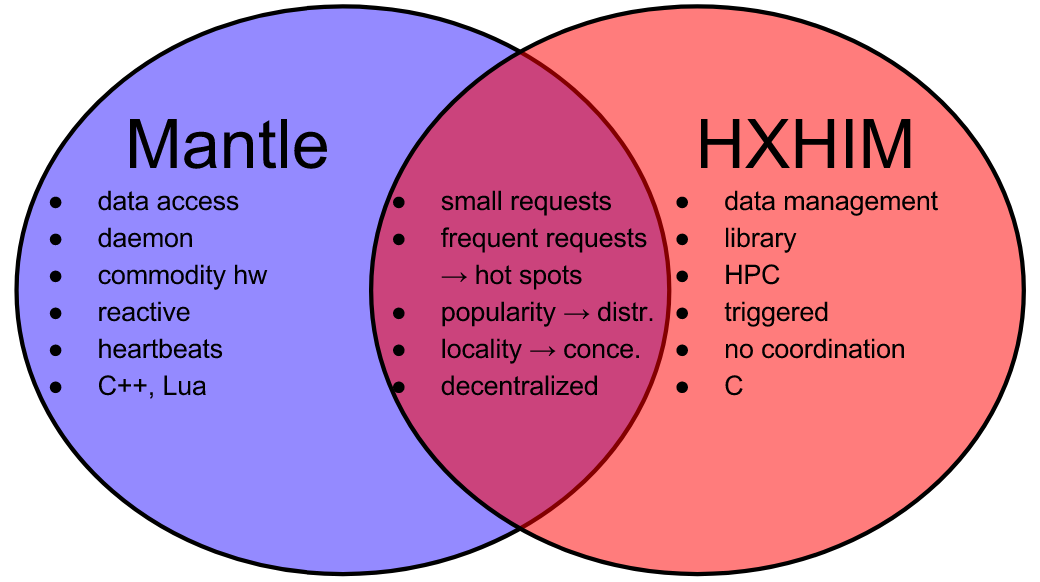
\includegraphics[width=19pc,angle=0]{figures/arch-comparison.png}\\
  \caption{Comparing the design goals and implementations of Mantle and HXHIM.}
  \label{fig:arch-comparison}
\end{figure}

